\documentclass[12pt]{article}

\usepackage{graphicx}
\usepackage[margin = 3 cm]{geometry}
\usepackage[english]{babel}
\usepackage[utf8x]{inputenc}
\usepackage{amsmath}
\usepackage[colorinlistoftodos]{todonotes}
\usepackage{listings}
\usepackage{float} %For image positioning
\usepackage{subcaption} %For even more image positioning
\usepackage[figurename=Fig.]{caption}
\usepackage{rotating}





\begin{document}
%%Forside



\begin{titlepage}

\newcommand{\HRule}{\rule{\linewidth}{0.5mm}} % Defines a new command for the horizontal lines, change thickness here

\center % Center everything on the page
 
%----------------------------------------------------------------------------------------
%	HEADING SECTIONS
%----------------------------------------------------------------------------------------

\textsc{\LARGE Aalborg Tekniske Gymnasium}\\[1.5cm] % Name of your university/college
\textsc{\Large Studieområde-projekt}\\[0.5cm] % Major heading such as course name
\textsc{\large Fysik A \& el-teknik A}\\[0.5cm] % Minor heading such as course title

%----------------------------------------------------------------------------------------
%	TITLE SECTION
%----------------------------------------------------------------------------------------

\HRule \\[0.4cm]
{ \huge \bfseries En fjernstyret kanon \& det skrå kast  }\\[0.4cm] % Title of your document
\HRule \\[1.5cm]
 
%----------------------------------------------------------------------------------------
%	AUTHOR SECTION
%----------------------------------------------------------------------------------------

\begin{minipage}{0.4\textwidth}
\begin{flushleft} \large
\emph{Forfatter:}\\
Nikolai \textsc{Bonderup}\\ % Your name
Sebastian \textsc{Lassen}\\
Lucas \textsc{Rasmussen}
\end{flushleft}
\end{minipage}
~
\begin{minipage}{0.4\textwidth}
\begin{flushright} \large
\emph{Vejleder:} \\
Pia \textsc{Thomsen} \\ % Supervisor's Name
Tom \textsc{Berthelsen}\\
\end{flushright}
\end{minipage}\\[2cm]

% If you don't want a supervisor, uncomment the two lines below and remove the section above
%\Large \emph{Author:}\\
%John \textsc{Smith}\\[3cm] % Your name

%----------------------------------------------------------------------------------------
%	DATE SECTION
%----------------------------------------------------------------------------------------

{\large \today}\\[2cm] % Date, change the \today to a set date if you want to be precise



\vfill % Fill the rest of the page with whitespace

\end{titlepage}



%%%%---------------------------------------------
%%Titelblad
%%%%---------------------------------------------
\subsection*{Titelblad}
\textbf{Projekttitel} Sensorer og datakommunikation\\
\textbf{Uddannelsessted og klasse} Aalborg tekniske Gymnasium, Q16\\
\textbf{Fag} Teknikfag, Elektronik A\\
\textbf{Projektperiode} x/x/2018 - x/1/2019\\
\textbf{Projektet udarbejdet af:}\\






%%%%---------------------------------------------
%%Rapport
%%%%---------------------------------------------
\renewcommand{\contentsname}{Indholdsfortegnelse}
\tableofcontents
\newpage

%%%%---------------------------------------------
%%Projektbeskrivelse
%%%%---------------------------------------------

%%Indledning
\newpage
%Dokument til indledningen
\section{Indledning}

Projektet ligger under studieområdet, hvilket her betyder at vi skal kombinere vores teknikfag med et af vores studieretningsfag. Vi har i gruppen valgt at bruge Fysik A, da dette virkede som det mest oplagte valg ift. bidragelse med projektrelevant teori. Projektet skal derfor også overholde forskellige krav fra SO, el-tek og fysik A, som bliver yderligere fremhævet i kravspecifikationen.\\

Vi har i gruppen besluttet os for at bygge en fjernstyret airsoft kanon, da dette produkt vil tilfredsstille alle de givne el-tek krav, samt at fysikteorien omkring det skrå kast kan bruges til at bestemme, hvor dets projektil vil ramme og hvor hurtigt det bevæger sig. Det kan gøres ved at måle, hvor langt kanonen skyder og hvilken vinkel løbet er peget op med, for så derefter at beregne mundingshastigheden vha. formler for det skrå kast. Dette kan så krydstjekkes med en målt projektilhastighed for, at opnå et fysikeksperiment udført med hjælp af elektriske komponenter.


%%Kravspecifikation
\newpage
\documentclass[12pt]{article}

\usepackage{graphicx}
\usepackage[margin = 3 cm]{geometry}
\usepackage[english]{babel}
\usepackage[utf8x]{inputenc}
\usepackage{amsmath}
\usepackage[colorinlistoftodos]{todonotes}
\usepackage{listings}
\usepackage{float} %For image positioning
\usepackage{subcaption} %For even more image positioning
\usepackage[figurename=Fig.]{caption}
\usepackage{rotating}


\begin{document}

%%Problemanalyse
\newpage
%Dokument til Projektanalyse
\subsection{Projektanalyse}

I dette projekt skal vi kombinere Fysik A og el-tek til et SO forløb. I projektet er der flere faglige mål som skal opfyldes indenfor området el-tek og fysik. Selve opgaven lyder på at gøre brug af de elementer som er at finde under kravspecifikationer. I problemanalysen skal disse elementer altså gennemgås og der skal vurderes, hvilket et af dem bliver det største “problem” at arbejde med.\\

Det mest udfordrende bliver at få skabt kommunikation mellem selve kanonen og et kontrolelement. Der skal være en modtager og afsender, måske endda en af hver på både kontrolmodul og kanon-modulet alt efter hvor avanceret arbejdet med denne del af projektet skal være.\\

Et andet udfordrende problem bliver, hvordan selve lade- og affyringsmekanismen skal hænge sammen så den kan virke ved fjernstyring. Her skal flere forskellige typer motorer styres præcist gennem bluetooth.


%%Forside



\begin{titlepage}

\newcommand{\HRule}{\rule{\linewidth}{0.5mm}} % Defines a new command for the horizontal lines, change thickness here

\center % Center everything on the page
 
%----------------------------------------------------------------------------------------
%	HEADING SECTIONS
%----------------------------------------------------------------------------------------

\textsc{\LARGE Aalborg Tekniske Gymnasium}\\[1.5cm] % Name of your university/college
\textsc{\Large Studieområde-projekt}\\[0.5cm] % Major heading such as course name
\textsc{\large Fysik A \& el-teknik A}\\[0.5cm] % Minor heading such as course title

%----------------------------------------------------------------------------------------
%	TITLE SECTION
%----------------------------------------------------------------------------------------

\HRule \\[0.4cm]
{ \huge \bfseries En fjernstyret kanon \& det skrå kast  }\\[0.4cm] % Title of your document
\HRule \\[1.5cm]
 
%----------------------------------------------------------------------------------------
%	AUTHOR SECTION
%----------------------------------------------------------------------------------------

\begin{minipage}{0.4\textwidth}
\begin{flushleft} \large
\emph{Forfatter:}\\
Nikolai \textsc{Bonderup}\\ % Your name
Sebastian \textsc{Lassen}\\
Lucas \textsc{Rasmussen}
\end{flushleft}
\end{minipage}
~
\begin{minipage}{0.4\textwidth}
\begin{flushright} \large
\emph{Vejleder:} \\
Pia \textsc{Thomsen} \\ % Supervisor's Name
Tom \textsc{Berthelsen}\\
\end{flushright}
\end{minipage}\\[2cm]

% If you don't want a supervisor, uncomment the two lines below and remove the section above
%\Large \emph{Author:}\\
%John \textsc{Smith}\\[3cm] % Your name

%----------------------------------------------------------------------------------------
%	DATE SECTION
%----------------------------------------------------------------------------------------

{\large \today}\\[2cm] % Date, change the \today to a set date if you want to be precise



\vfill % Fill the rest of the page with whitespace

\end{titlepage}



%%Problemformulering
\newpage
%Dokument til Projektformulering
\section{Projektformulering}

%%Problemformulering
\newpage
%Dokument til projektafgrænsningen
\section{Projektafgrænsning}

Vi har planlagt at arbejde med en kanon som skal kunne rotere 360 grader, samt have et vinkelinterval til affyring af kanonen på mindst 100 grader. Den fjernstyrede kanon skal være i stand til at modtage information fra et kontrolmodul. Dette skal ske ved brug af en bluetooth enhed eller et andet trådløst kommunikationsmodul. Der skal altså laves en mikrocontroller som kan styre kanonen gennem disse trådløse moduler ved at få kommandoer fra et kontrolmodul.\\

\begin{figure}[H]
\centering
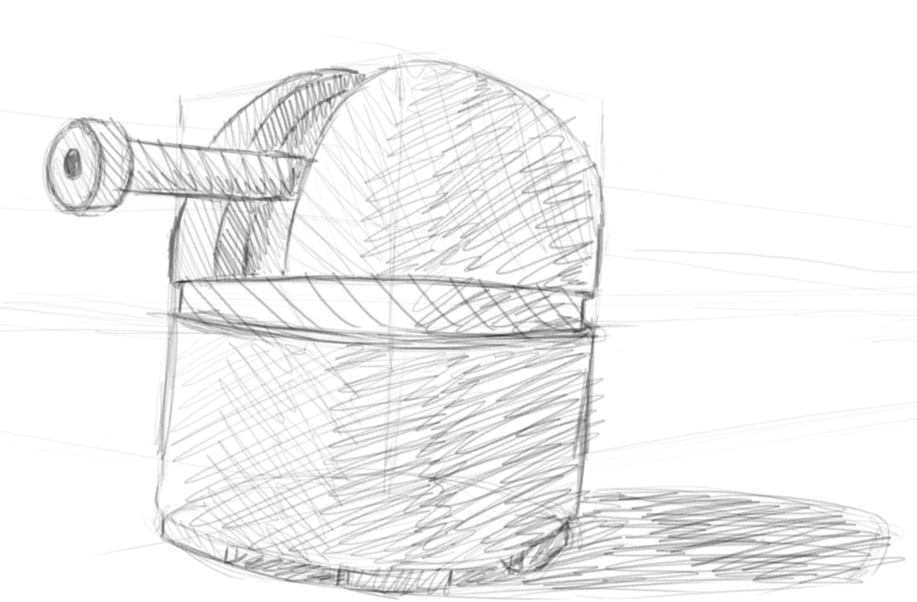
\includegraphics[scale=0.4]{Billeder/Koncept_turret.png}
\caption{Koncept af kanon.}
\label{fig:KonceptKanon}
\end{figure}

Selve kanons affyringsmekanisme laves enten med en “airsoft” pneumatisk gearkasse, hvor en DC motor bruges til at trække en fjeder op. Denne fjeder laver et lufttryk i gearkassens trykkammer som kan bruges til at skyde et projektil afsted. Selve robottens krop laves vha. 3D print af de enkelte komponenter, der sættes sammen med enten lim eller skruer. \\

Til udarbejdningen af det fysikvidenskabelige dokumentation kan der påmonteres forskellige accelerometerer, som kan bruges til at bestemme skydevinklen. Derudover kan der alternativt måles, hvor langt projektilet bliver affyret for så, at kunne beregne dets hastighed, hvis affyringsvinklen er kendt.

\begin{figure}[H]
\centering
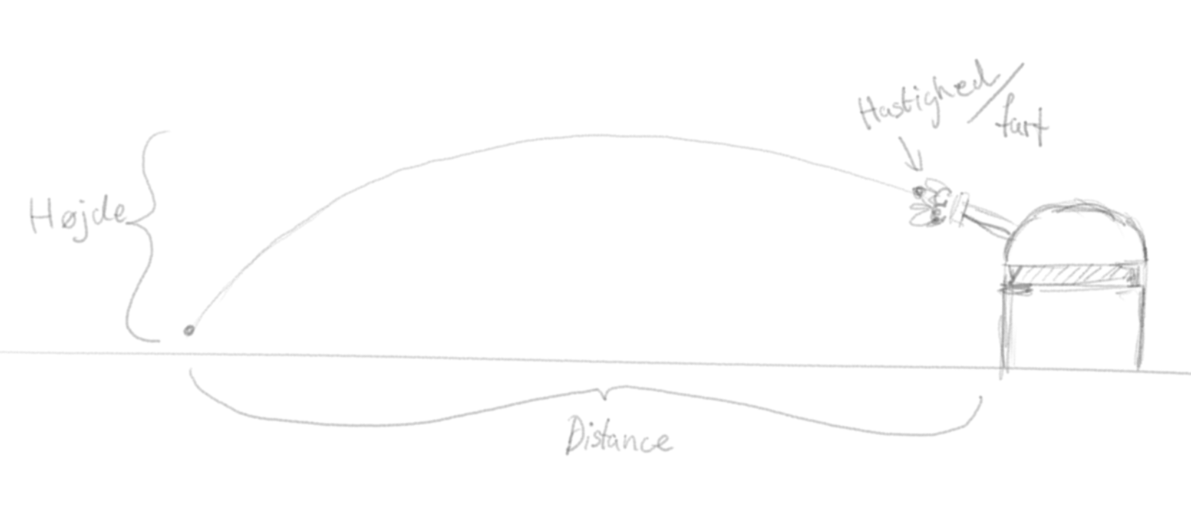
\includegraphics[scale=0.4]{Billeder/Fysik_koncept.png}
\caption{Fysik relevant til kanonen.}
\label{fig:FysikKoncept}
\end{figure}

%%Kravspecifikation
\newpage
%Dokument til kravspecifikationer
\section{kravspecifikationer}

De opstillede krav fra el-tek:

Der skal bruges en “interrupt” (HW - Kontakt, SW - Timer).
Der skal altså i projektet bruges enten en kontakt eller timer i vores kredsløb. Det er påkrævet at denne har en relevant betydning for selve kredsløbet og ikke har en meningsløs funktion.

Der skal være et sensor input: analog til digital konvertering.
Dette forstås som at der skal bruges en type sensor, som måler noget analogt, der derefter kan oversættes til noget digitalt vha. en mikroprocessor. Dette kunne for eksempel være en afstandssensor.

Digital til Analog konvertering.
Dette vil ved brug af Arduino i de fleste tilfælde være at bruge et PWM signal til kontrol af et elektronisk element.

Der skal bruges datakommunikation (til pc, viserinstrument eller trådløst element).
Dette ville være en form for input/output type af kontrol i forhold til vores produkt. Her skal gruppen kunne give en eller anden form for ordre til produktet og produktet skal så udføre en bestemt handling. Dette kunne opfyldes ved at styre kanonens vinkel med en controller vha. bluetooth.

Et print til en mikrocontroller.
Der skal til produktet bruges et selvproduceret mikrocontrollerprint. Denne microcontroller skal kunne styre en af hovedelementerne i selve produktet for at opfylde kravet om at have en relevant funktion.

Udover de specifikke krav skal der også indrages relevant fysikteoretisk arbejde, som udmunder i afleveringen af videnskabelig dokumentation vedrørende det valgte fysikteori og el-tek produkt.


\end{document}

%%%%---------------------------------------------
%%Fysik Rapport
%%%%---------------------------------------------
\section{Systembeskrivelse}



\subsection{Fysik teori}

\begin{figure}[H]
\centering
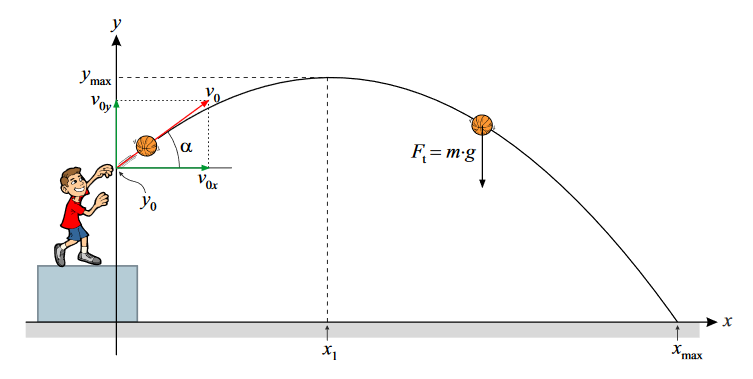
\includegraphics[scale=0.7]{Billeder/skrakast.png}
\caption{Skitse af det skraa kast. Figuren stammer fra \url{http://www.matematikfysik.dk/fys/noter_tillaeg/tillaeg_det_skraa_kast_uden_luftmodstand.pdf}}.
\label{fig:Resultatbehandling3}
\end{figure}

\textbf{Teoretisk udledning af formler til det skrå kast}\\
Begyndelseshastigheden for et kast er givet ud fra vektoren $v_{0}$ og vinklen a, det betyder altså at hastighedsvektorens komposanter kan findes ved:\\

\begin{center}
\begin{math}
\centering
v_{x} = v_{0} \cdot cos(a) \quad \textrm{og} \quad v_{y} = v_{0} \cdot sin(a)
\end{math}
\end{center}

Samtidigt vides det at x- og y-slut kan skrives som to bevægelsesligninger:\\

\begin{center}
\begin{math}
\centering
y = -\dfrac{1}{2} \cdot g \cdot t^{2} + v_{y} \cdot t + y_{0}
\end{math}
\end{center}



Hvor dette er formlen for strækning inden for faget kinematik, omskrevet til at passe på y-aksen i det skrå kast. Her skiftes strækningen ud med y og accelerationen med g, da det er tyngdeaccelerationen som kastet arbejder imod:\\

\begin{center}
\begin{math}
\centering
s = -\dfrac{1}{2} \cdot g \cdot t^{2} + v_{0} \cdot t + s_{0} 
\end{math}
\end{center}

x er derved givet ved konstant hastighed, denne får altså ligningen:\\

\begin{center}
\begin{math}
\centering
x = v_{x} \cdot t
\end{math}
\end{center}

Hvor denne er omskrevet fra formlen for konstant hastighed:\\

\begin{center}
\begin{math}
\centering
v = \dfrac{\Delta s}{\Delta t}
\end{math}
\end{center}




Hvor der isoleres for strækningen:\\

\begin{center}
\begin{math}
v = \dfrac{\Delta s}{\Delta t} \longrightarrow \Delta s = v \cdot \delta t
\end{math}
\end{center}

Dette giver altså to ligninger for x- og y-slut nr komposanterne indsættes:\\

\begin{center}
\begin{math}
x_{slut} = v_{0} \cdot cos(a) \cdot t
\end{math}
\end{center}

og\\

\begin{center}
\begin{math}
y_{slut} = -\dfrac{1}{2} \cdot g \cdot t^{2} + v_{0} \cdot sin(a) \cdot t + y_{0}
\end{math}
\end{center}

\textbf{Bestemmelse af  $x_{slut}$}\\
I vores forsøg kender vi hverken tiden eller $x_{slut}$. Tiden kan dog bestemmes.\\

Det vides at $y_{slut}$ er lig $y_{0}$, da planet forsøget er udført på er ensartet, dette vil altså sige, at både $y_{o}$ og $y_{slut}$ er lig 0. Dette kan altså sættes ind i ligningen for $y_{slut}$ og der kan isoleres for t:\\

\begin{center}
\begin{math}
0 = -\dfrac{1}{2} \cdot g \cdot t^{2} + v_{y} \cdot t + y_{0} \longrightarrow t = \dfrac{v_{y} + \sqrt{2 \cdot g \cdot y_{0} + y^{2}_{y}}}{g}
\end{math}
\end{center}

Den tidligere bestemte y komposant kan indsættes så alle variabler kendes:\\

\begin{center}
\begin{math}
t = \dfrac{v_{0} \cdot sin(a) + \sqrt{2 \cdot g \cdot y_{0} + y^{2}_{y}}}{g}
\end{math}
\end{center}

\textbf{Opsat som vektorfunktion}\\
Vektorfunktioner er givet ud fra en ligning for bevægelsen på x-aksen og bevægelsen på y-aksen:

\begin{center}
\begin{math}
\overrightarrow{r}(t) = 
\begin{pmatrix}
x(t)\\
y(t)
\end{pmatrix}
\end{math}
\end{center}

Da bevægelser er beskrevet ved brug af vektorere opsættes skuddet som en vektorfunktion:

\begin{center}
\begin{math}
\overrightarrow{r}(t) = 
\begin{pmatrix}
v_{0} \cdot cos(a) \cdot t\\
- \dfrac{1}{2} \cdot g \cdot t^{2} + v_{0} \cdot sin(a) \cdot t + y_{0}
\end{pmatrix}
\end{math}
\end{center}

\subsection{Forsøg}
\subsubsection{Apparaturliste}
\begin{itemize}
\item 2x opsætnings stativer
\item 1x BT5 A5 Elektrisk Airsoft Gevær
\item 1x LiDAR af typen Leica “Disto D5”
\item 1x Tomstok
\end{itemize}

\subsubsection{Fremgangsmåde}

\begin{figure}[H]
\centering
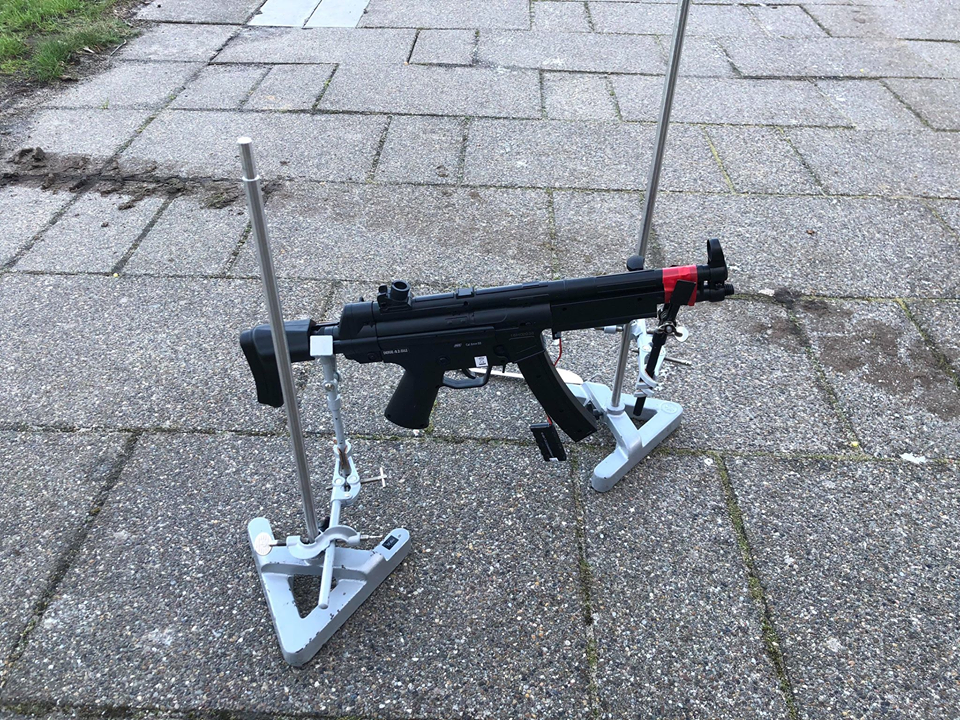
\includegraphics[scale=0.4]{Billeder/Opstilling.png}
\caption{Forsogsopstilling.}
\label{fig:Opstilling}
\end{figure}


\begin{enumerate}
\item Først opsættes det elektriske airsoft gevær på en sådan måde at vinklen er let at ændre, denne opsætning ses på figur \ref{fig:Opstilling}.

\item Der indstilles en vinkel. 
\begin{enumerate}
\item Højden mellem de to monteringspunkter og jorden måles.
\item Der måles en afstand mellem de to monteringspunkter, dette er en hypotenuse mellem de to monteringspunkter.
\item det lave monteringspunkt trækkes fra det høje, og nu er en modstående katete til den ønskede vinkel fundet.
\item Bestem brugt vinkel ud fra sinus beregning.
\end{enumerate}

\item Skud affyres.

\item Afstanden fra skuddets første kontaktpunkt med jorden hen til gevær-opstillingen ved hjælp af LiDAR.

\item Der tages tre målinger for hver vinkel.
\end{enumerate}

\subsubsection{Resultatbehandling}

For at undersøge hypotesen om, hvorvidt det skrå kast er en god model til at beskrive airsoft-geværets skud vil vi sammenligne de teoretiske beregninger med det målte data. Til at gøre dette har vi sammenlignet den teoretisk beregnede $x_{slut}$ med den gennemsnitlige målte $x_{slut}$ ($x_{1}$, $x_{2}$ osv.) for hver vinkel vi har udført målinger med. Den grønne kurve og det sorte punkt er de teoretiske værdier, mens de blå punkter er det målte data.

\begin{figure}[H]
\centering
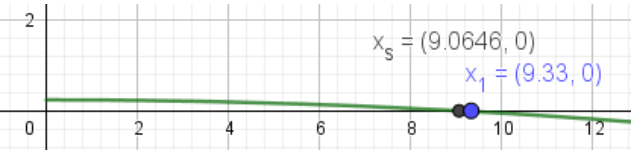
\includegraphics[scale=0.7]{Billeder/Resultatbehandling1.png}
\caption{Korsel 1. Vandret skudvinkel, haevet 0,23 m.}
\label{fig:Resultatbehandling1}
\end{figure}

Som det kan ses på figur \ref{fig:Resultatbehandling1} skyder geværet meget tæt på den teoretiske længde når skudvinklen er vandret. Det betyder at den kendte funktion for det skrå kast uden luftmodstand er en god model til at beskrive skud med denne vinkel, da den ville kunne ramme en skive på størrelse med et menneske, hvis den er indstillet vha. den teoretiske kurve.

\begin{figure}[H]
\centering
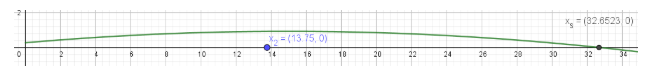
\includegraphics[scale=0.7]{Billeder/Resultatbehandling2.png}
\caption{Korsel 2. Skudvinkel på 5 grader, haevet 0,27 m.}
\label{fig:Resultatbehandling2}
\end{figure}

Som det kan ses på figur \ref{fig:Resultatbehandling2} burde skuddet flyve mere end tredobbelt så langt som før ved denne vinkel, men at dette ikke sker i praksis. For at konstruere en mere beskrivende kurve for skuddet ved 5 grader, kan man modificere kurven for det skrå kast ved at omskrive y(t)-leddet så den hælder dobbelt så meget.

\begin{figure}[H]
\centering
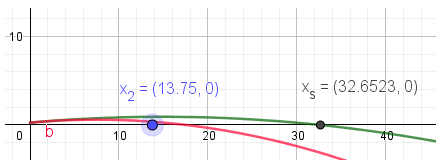
\includegraphics[scale=0.7]{Billeder/Resultatbehandling3.png}
\caption{Korsel 2. Den rode linje angiver den modificerede kurve.}
\label{fig:Resultatbehandling3}
\end{figure}

\begin{center}
\begin{math}
\overrightarrow{r}(t) = 
\begin{pmatrix}
v_{0} \cdot cos(a) \cdot t\\
- \dfrac{1}{2} \cdot g \cdot t^{2} + v_{0} \cdot sin(a) \cdot t + y_{0}
\end{pmatrix}
\end{math}
\end{center}

\begin{center}
\begin{math}
\overrightarrow{r}(t) = 
\begin{pmatrix}
v_{0} \cdot cos(a) \cdot t\\
- \dfrac{1}{2} \cdot g \cdot t^{2} + v_{0} \cdot sin(a) \cdot t + y_{0}
\end{pmatrix}
\end{math}
\end{center}

\begin{center}
\begin{math}
\overrightarrow{r}(t) = 
\begin{pmatrix}
v_{0} \cdot cos(a) \cdot t\\
-1 \cdot g \cdot t^{2} + v_{0} \cdot sin(a) \cdot t + y_{0}
\end{pmatrix}
\end{math}
\end{center}

Som det kan ses på figur \ref{fig:Resultatbehandling3} får kurven en dobbelt så stor hældning ved at multiplikere y(t)-leddet med 2, så $-\dfrac{1}{2}$ bliver til $-1$.

\begin{figure}[H]
\centering
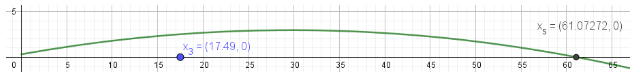
\includegraphics[scale=0.7]{Billeder/Resultatbehandling4.png}
\caption{Korsel 3. Skudvinkel på 10 grader, haevet 0,31 m}
\label{fig:Resultatbehandling4}
\end{figure}

Igen viser figur \ref{fig:Resultatbehandling4} at den teoretiske værdi er mange gange større end den praktiske. Denne gang viser kurven at skuddet burde flyve mere end tredobbelt så langt som tidligere, hvilket peger i retning af at som skudvinklen bliver større, og dermed også længden af skuddets bane, bliver 
den praktiske skudlængde eksponentielt mindre sammenlignet med den teoretiske.\\

Ud fra det kan vi opstille en mere generel kurve til vores skud, som inkorporerer en stigende hældning i takt med at skudvinklen stiger. Dette kan gøres ved at observere, hvordan den teoretiske værdi svinger mere fra den praktiske jo større skudvinklen er. \\

For 0 grader:	$x_{teori} = 1x_{praktisk} $\\
For 5 grader:	$x_{teori} = 2x_{praktisk} $\\
For 10 grader:	$x_{teori} = 3x_{praktisk} $\\
For 15 grader:	$x_{teori} = 4x_{praktisk} $\\[0.5cm]

For n grader: $ x_{teori} \approx ((\dfrac{n}{5})+1) $\\[0.5cm]

For at opsætte en kurve som følger dette princip, kan vi modificere x(t) så kurvens hældning bliver kraftigere i takt med at skudvinklen stiger.\\

\begin{center}
\begin{math}
x(t) = v_{0} \cdot cos(a) \cdot t
\end{math}
\end{center}

\begin{center}
\begin{math}
x(t) = \dfrac{v_{0} \cdot cos(a) \cdot t}{\dfrac{a}{5} + 1}
\end{math}
\end{center}

\begin{figure}[H]
\centering
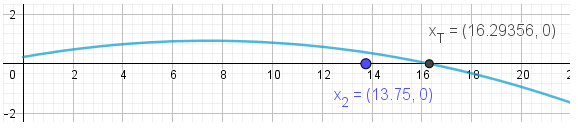
\includegraphics[scale=0.7]{Billeder/Resultatbehandling5.png}
\caption{Den nye funktions slutpunkt sammenlignet med maalepunktet ved 5 grader.}
\label{fig:Resultatbehandling5}
\end{figure}

Som det kan ses på figur \ref{fig:Resultatbehandling5} er der stadig en forskel på ca. 2,5 meter mellem de to nedslagspunkter. Denne forskel kan kraftigt formindskes ved at lægge 1,5 til i stedet for 1 i x(t).\\

\begin{center}
\begin{math}
x(t) = \dfrac{v_{0} \cdot cos(a) \cdot t}{\dfrac{a}{5} + 1.5}
\end{math}
\end{center}

For at undersøge om den nye kurve beskriver skuddene på $ > 5 $ grader mere præcist, kan vi sammenligne dens slutpunkt med målepunkterne. Noter at $ x_{T} $ er det nedslagspunkt kurven forudsiger, hvorimod $x_{2}$, $x_{3}$ etc. er målepunkter.\\

\begin{figure}[H]
\centering
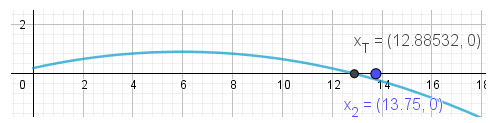
\includegraphics[scale=0.7]{Billeder/Resultatbehandling6.png}
\caption{Den nye kurve og maalepunktet til 5 grader.}
\label{fig:Resultatbehandling6}
\end{figure}

\begin{figure}[H]
\centering
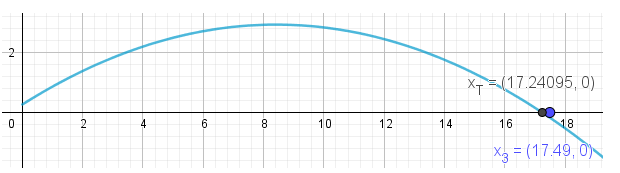
\includegraphics[scale=0.7]{Billeder/Resultatbehandling7.png}
\caption{Den nye kurve og maalepunktet til 10,15 grader.}
\label{fig:Resultatbehandling7}
\end{figure}

\begin{figure}[H]
\centering
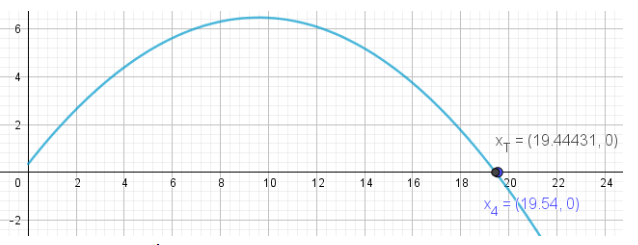
\includegraphics[scale=0.7]{Billeder/Resultatbehandling8.png}
\caption{Den nye kurve og maalepunktet til 15,53 grader.}
\label{fig:Resultatbehandling8}
\end{figure}

Som det kan ses på figur \ref{fig:Resultatbehandling6} , \ref{fig:Resultatbehandling7} og \ref{fig:Resultatbehandling8} passer den nye kurve og dens nedslagspunkt meget præcist på det beregnede. Modellen beskriver altså, hvordan vores airsoft-gevær skyder meget mere præcist end det skrå kast, da denne tager hensyn til vinklen samt konstanten 1,5, der bliver lagt til. Konstanten og hensynet til vinklen bruges altså til at tage luftmodstanden med i beregningen, da denne er forskellen på forsøgsdataet og det skrå kasts teoretiske beregninger.\\[0.5cm]

Kurven til vores airsoft-geværs skud bliver altså beskrevet ved:\\

\begin{center}
\begin{math}
\overrightarrow{r}(t) = 
\begin{pmatrix}
x(t)\\
y(t)
\end{pmatrix}
=
\begin{pmatrix}
\dfrac{v_{0} \cdot cos(a) \cdot t}{\dfrac{a}{5} + 1.5}\\
- \dfrac{1}{2} \cdot g \cdot t^{2} + v_{0} \cdot sin(a) \cdot t + y_{0}
\end{pmatrix}
\end{math}
\end{center}


\subsubsection{Diskussion}

Mange faktorer har haft en indflydelse på indsamlingen af måledata til dette forsøg. Først og fremmest var det nødvendigt at lave forsøget udenfor, da geværet både skyder langt og højt. Dette skaber problemer i forhold til vind, da kuglerne er meget lettere. Dette kan blandt andet være grunden til at de længere skud har større variation i hvor de lander, da de har haft længere tid til at blive påvirket af eventuelle vindstød.\\

Samtidigt var det svært at se præcis hvor kuglerne landede da de er små og flyver relativt hurtigt. (Mundingshastigheden er cirka 41 m/s og kuglernes diameter er 6 mm). Dette problem løste vi dog ved at bruge en sandkasse. Her hoppede kuglerne nemlig sjældent efter de ramte jorden og blev som regel liggende hvor de ramte. Dette gjorde selve måle-arbejdet betydeligt meget lettere.\\

Inden vi opsatte vores egen vektorfunktion som model til skuddene, afprøvede vi en anden kendt model for det skrå kast med luftmodstand\footnote{\url{ http://www.matematiksider.dk/projekter/skraakast.pdf}}.\\

\begin{center}
\begin{math}
\overrightarrow{r}(t) = 
\begin{pmatrix}
x(t)\\
y(t)
\end{pmatrix}
=
\begin{pmatrix}
\dfrac{v_{0} \cdot cos(a) \cdot t}{\dfrac{a}{5} + 1.5}\\
- \dfrac{1}{2} \cdot g \cdot t^{2} + v_{0} \cdot sin(a) \cdot t + y_{0}
\end{pmatrix}
\end{math}
\end{center}

Vi fandt dog hurtigt ud af at denne kun er egnet når man arbejder med objekter, der enten er meget tungere eller bevæger sig markant langsommere, da den overestimerer luftmodstanden så meget ved vores skud, at nedslagspunktet ligger indenfor de første 0,5 meter ved alle vinkler.


















\newpage

\subsection{Elektriske kredsløb}
I dette projekt er der i alt 2 forskellige elektriske kredsløb ( hvis man ignorere de isoleret kredsløb, som bliver skabt pga. Brugen af H-broer og hardball pistol). Kredsløb \#1 er kredsløbet som kan findes på selve kanon. Dette kredsløb styrer kanonens bevægelse vha. Motorer og sensorer. Kredsløb \#2 er kredsløbet som findes på kontrolleren. Dette kredsløb bruges til at styrer kanonen gennem et bluetooth signal fra kredsløb \#2 til kredsløb \#1. \\

%Kredsløb 1
\textbf{{\normalsize Kredsløb \#1}}

\begin{figure}[H]
\centering
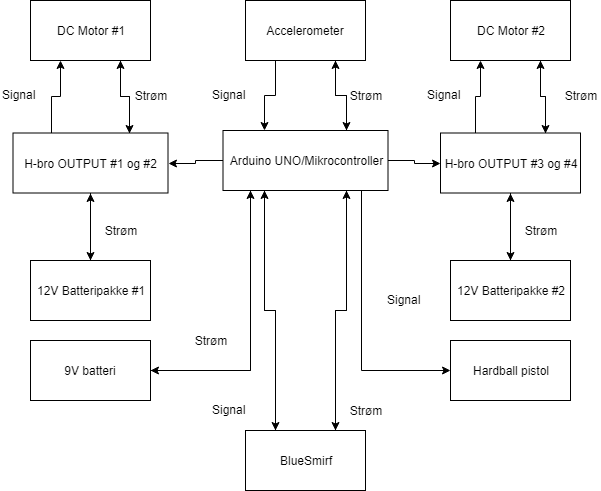
\includegraphics[scale=0.8]{Billeder/Kredsloeb1.png}
\caption{Blokdiagram af kredsløb \#1.}
\label{fig:Blokdiagram1}
\end{figure}


\begin{figure}[H]
\centering
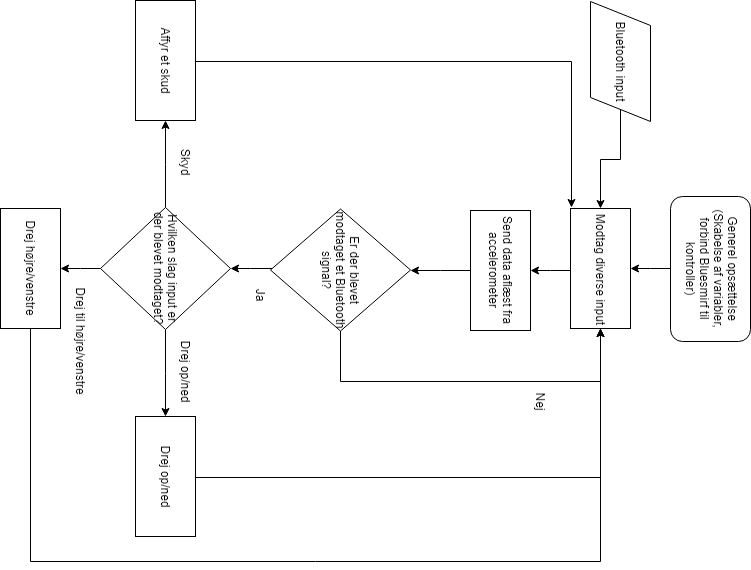
\includegraphics[scale=0.8, angle = 90]{Billeder/Flowchart1.png}
\caption{Flowdiagram af kredsløb \#1.}
\label{fig:Flowdiagram1}
\end{figure}

\newpage
\textbf{Systemdele}
\begin{itemize}
	\item Arduino UNO
\begin{itemize}
\item På blokdiagrammet (Fig. \ref{fig:Blokdiagram1}) kan det ses, at Arduinonen er forbundet til næsten alle elektroniske elementer i robotten. 
\end{itemize}

	\item 9V batteri
\begin{itemize}
\item Dette 9 volts batteri fungere som Arduinoens strømforsyning.
\end{itemize}

	\item 12V batteripakke \#1
\begin{itemize}
\item Denne batteripakke fungere som stepper motor \#1’s strømforsyning.
\end{itemize}

	\item 12V batteripakke \#2
\begin{itemize}
\item Denne batteripakke fungere som stepper motor \#2’s strømforsyning.
\end{itemize}

	\item H-bro ( LN298 ) \#1
\begin{itemize}
\item H-bro \#1 er forbundet til stepper motor \#1 og 12V batteripakke \#1. Derudover bliver H-broen kontrolleret af en Arduino, som ikke er i kredsløb med batteripakke \#1.
\end{itemize}

	\item H-bro ( LN298 ) \#2
\begin{itemize}
\item H-bro \#2 er forbundet til stepper motor \#2 og 12V batteripakke \#2. Derudover bliver H-broen kontrolleret af en Arduino, som ikke er i kredsløb med batteripakke \#2.
\end{itemize}

	\item Stepper Motor \#1
\begin{itemize}
\item Stepper \#1 er forbundet til 12V batteripakke \#1 via. H-bro \#1. Derudover er stepper motoren kontrolleret af H-bro \#1. 
\end{itemize}

	\item Stepper Motor \#2
\begin{itemize}
\item Stepper \#2 er forbundet til 12V  batteripakke \#2 via. H-bro \#2. Derudover er stepper motoren kontrolleret af H-bro \#2
\end{itemize}

	\item Accelerometer
\begin{itemize}
\item Accelerometeret er forbundet til Arduinoen, som den desuden også modtager strøm fra.
\end{itemize}

	\item Hardball pistol 
\begin{itemize}
\item Hardball pistolen indgår også i det elektriske kredsløb. Hardball pistolens skyde mekanism bliver kontrolleret af Arduinoen. I selve hardball pistolen findes der også et elektrisk kredsløb, dog er delene til dette kredsløb ikke beskrevet i blokdiagrammet, da det ikke er et selv fabrikeret elektrisk komponent. 	
\end{itemize}

\item BlueSmirf
\begin{itemize}
\item BlueSmirf modulet modtager strøm fra Arduinoen. Derudover kommunikere BlueSmirf modulet med Arduinoen.
\end{itemize}

\end{itemize}



%Kredsløb 2
\textbf{{\normalsize Kredsløb \#2}}

\begin{figure}[H]
\centering
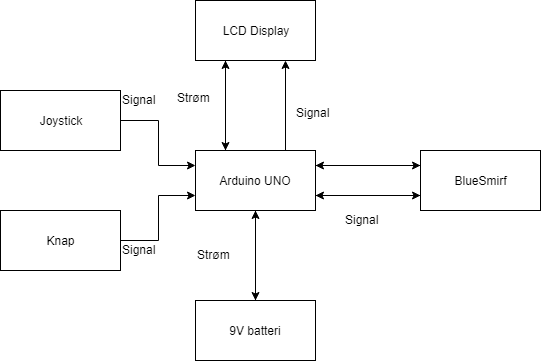
\includegraphics[scale=0.8]{Billeder/Kredsloeb2.png}
\caption{Blokdiagram af kredsløb \#2.}
\label{fig:Blokdiagram2}
\end{figure}


\begin{figure}[H]
\centering
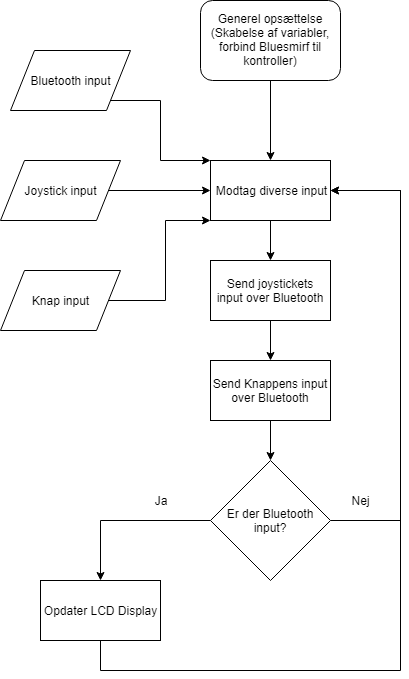
\includegraphics[scale=0.8]{Billeder/Flowchart2.png}
\caption{Flowdiagram af kredsløb \#2.}
\label{fig:Flowdiagram2}
\end{figure}

\newpage
\textbf{Systemdele}
\begin{itemize}
	\item Arduino UNO
\begin{itemize}
\item På blokdiagrammet (Fig. \ref{fig:Blokdiagram2}) kan det ses, at Arduinonen er forbundet til alle elektroniske elementer. 
\end{itemize}

	\item 9V batteri
\begin{itemize}
\item Dette 9 volts batteri fungere som Arduinoens strømforsyning.
\end{itemize}

	\item Joystick
\begin{itemize}
\item Joysticket er forbundet til Arduinoen, som måler strømmen der løber gennem joysticket.
\end{itemize}

	\item Knap
\begin{itemize}
\item Knappen er forbundet til Arduinoen, som måler strømmen der løber gennem knappen.
\end{itemize}

	\item BlueSmirf
\begin{itemize}
\item BlueSmirf modulet modtager strøm fra Arduinoen. Derudover kommunikere BlueSmirf modulet med Arduinoen.
\end{itemize}

	\item LCD Display
\begin{itemize}
\item LCD Display modulet er forbundet til Arduinoen og modtager også strøm fra Arduinoen. 
\end{itemize}

\end{itemize}








\newpage

\section{Konklusion}
\newpage

\section{Litteraturliste}
\emph{Teknisk Matematik} af Preben Madsen, 4. Udgave. \\[0.5cm]
\emph{Orbit B} af Per Holck, Jens Kraaer og Birgitte Merci Lund. \\[0.5cm]
\url{http://www.matematikfysik.dk/fys/noter_tillaeg/tillaeg_det_skraa_kast_uden_luftmodstand.pdf} af \url{http://www.matematikfysik.dk}. Senest læst den 19/12/2018.\\[0.5cm]
\url{http://www.matematiksider.dk/projekter/skraakast.pdf} af \url{http://www.matematiksider.dk}. Senest læst den 19/12/2018







\newpage

\section*{Bilag}




\end{document}
